\section{Specification}\label{sec:specification}
The following chapter describes the system specification.
The specification is derived from the requirements in the project description
as well as the discussions with the stakeholder.
Assumptions and constraints are described in the following sections and were validated by
the defined product owner and the stakeholder.

\subsection{System Delimitation}\label{subsec:system-delimination}
The system delimitation is split into the static system environment described in \fullref{subsubsec:system_environment}
and the dynamic process environment described in \fullref{subsubsec:process_environment}.

\subsubsection{System Environment}\label{subsubsec:system_environment}
The static system environment is split into the three contexts \textit{System}, \textit{System context}, and \textit{Out of scope}.\ \textit{System} includes the application
as well as any software dependencies.
The \textit{System context} includes people or objects which have an influence on the application.\ \textit{Out of scope} describes particularly
what could have an influence on the application but has been deliberately excluded by the project team (see~\fullref{subsubsec:pre_conditions_and_boundaries}). \\~\\
\textit{System}:
\begin{itemize}
    \item Frontend (User interaction)
    \item LaTeX and pgfplots
    \item WAV file analyzer
\end{itemize}
\textit{System context}:
\begin{itemize}
    \item Stakeholder (tutor)
    \item User
    \item Noise producers
    \item Lärmliga
    \item Recording Device
\end{itemize}
\textit{Out of scope}:
\begin{itemize}
    \item Integration in legal complaints
\end{itemize}

\begin{figure}[H]
    \centering
    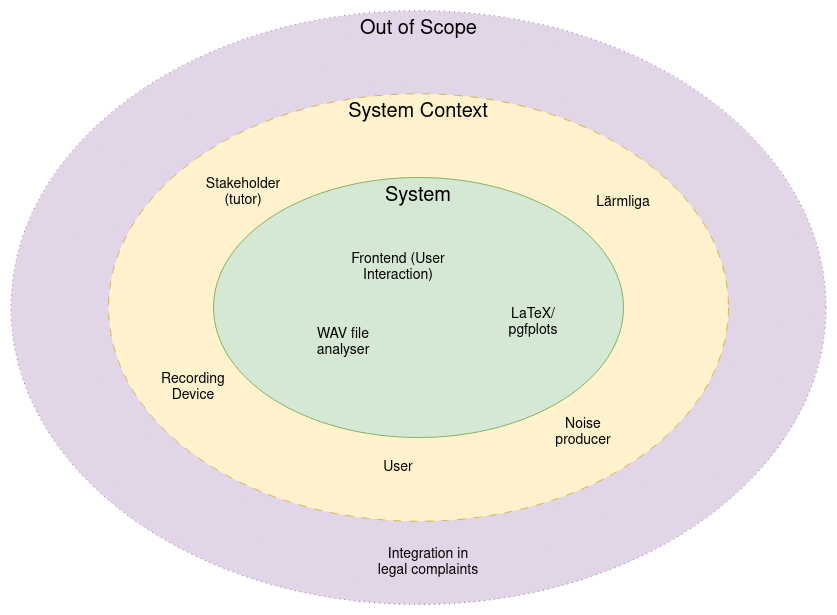
\includegraphics[width=1\textwidth]{../assets/system_environment.png}
    \caption{System Environment}\label{fig:system-environment}
\end{figure}

\subsubsection{Process Environment}\label{subsubsec:process_environment}
As in the previous chapter \fullref{subsubsec:system_environment}, the process environment is also split into \textit{System}, \textit{System context}, and \textit{Out of scope}. \\~\\
\textit{System}:
\begin{itemize}
    \item Selecting (uploading) a WAV file
    \item WAV file analysis (validation, parsing, conversion to absolute db values, threshold filtering)
    \item Plotting analysis result (LaTeX / pgfplots) and PDF generation
\end{itemize}
\textit{System context}:
\begin{itemize}
    \item Recording noise
    \item Producing noise
\end{itemize}
\textit{Out of scope}:
\begin{itemize}
    \item Device calibration (see \fullref{subsubsec:pre_conditions_and_boundaries})
\end{itemize}

\begin{figure}[H]
    \centering
    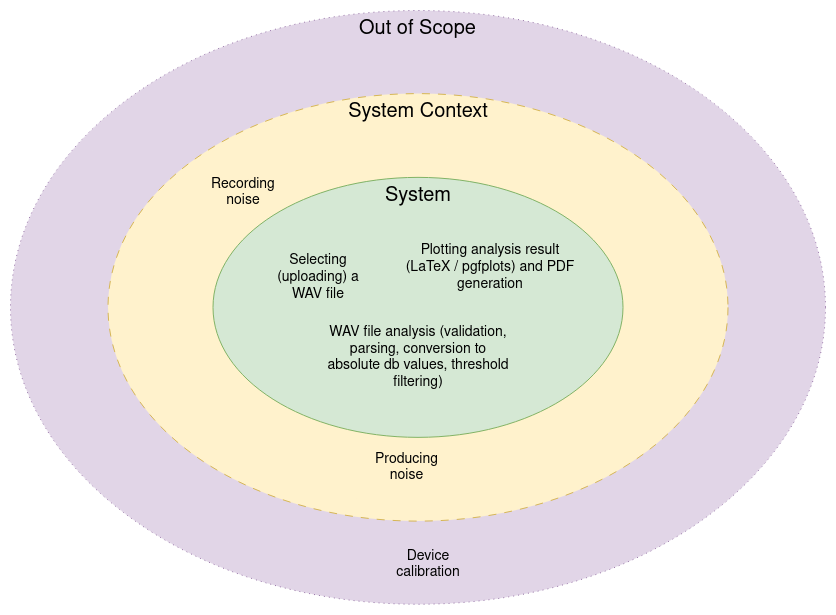
\includegraphics[width=1\textwidth]{../assets/process_environment.png}
    \caption{Process Environment}\label{fig:process-environment}
\end{figure}

\subsection{Requirements}\label{subsec:requirements}
In the following section the requirements are detailed. Also, the project boundaries and pre-conditions are described.

\subsubsection{Functional requirements}\label{subsubsec:functional_requirements}
The project team identified the following functional requirements:
\begin{table}[H]
    \centering
    \begin{tabularx}{\textwidth}{c X c c c}
        \toprule
        \textbf{ID} & \textbf{Requirement}                                                                                                    & \textbf{Priority} \\
        \midrule
        R1          & Allow users to upload a WAV audio file.                                                                                 & MUST              \\
        \midrule
        R2          & Validate the uploaded file to ensure it is in WAV format, providing an error message if it is not.                      & MUST              \\
        \midrule
        R3          & Analyze the uploaded WAV file and calculate the noise level in decibels (dB).                                           & MUST              \\
        \midrule
        R4          & Allow users to download the plotted noise data as an image or PDF.                                                      & MUST              \\
        \midrule
        R5          & Allow users to input metadata for the audio file, such as location, date, and time.                                     & MUST              \\
        \midrule
        R6          & Plot the noise level data over time, with the x-axis representing time and the y-axis representing noise level (in dB). & MUST              \\
        \midrule
        R7          & Generate a PDF report including the plotted noise data and user input metadata.                                         & MUST              \\
        \midrule
        R8          & Provide clear feedback and error messages.                                                                              & SHOULD            \\
        \midrule
        R9          & Intuitive and responsive UI for selecting files, configuring options, and viewing results.                              & SHOULD            \\
        \midrule
        R10         & Allow the user to configure custom thresholds for noise levels.                                                         & COULD             \\
        \midrule
        R11         & Allow the user to change the language of the application.                                                               & COULD             \\
        \bottomrule
    \end{tabularx}
    \caption{Functional Requirements}\label{table:functional_requirements}
\end{table}

\subsubsection{Pre-Conditions and Boundaries}\label{subsubsec:pre_conditions_and_boundaries}
Research done by the project team has revealed that reading absolute decibel values from WAV files is more difficult than anticipated.
The reason for this is that normal consumer microphones are not calibrated for scientifically accurate measurements\cite{stackoverflow_spl}. Furthermore, it is trivial for a user
to increase the volume of a WAV file using free, easy-to-use software like Audacity\cite{audacity,audacity_amplify}.
Therefore, the project team has decided on a tentative working hypothesis together with the Stakeholder. \\~\\
Pre-Conditions:
\begin{itemize}
    \item The user must use a properly calibrated microphone or use a phone app which has built-in calibrations like Decibel X\cite{decibelx_ios}\cite{decibelx_android}.
    \item The user must have a way to export their audio recording as a WAV file.
    \item The user must have access to a web browser capable of running WebAssembly.
    \item The user must not edit the exported WAV file in any way except to decrease the length of the recording.
\end{itemize}
Boundaries:
\begin{itemize}
    \item The application supports only the analysis of pre-calibrated, unedited WAV files.
    \item The application supports only single-channel WAV files.
    \item The application does not allow generating a legal complaint or directly integrating its output in a legal complaint.
    \item The user is presumed to be using properly calibrated equipment.
          There is no validation done in the application to ensure proper calibration.
    \item The user is presumed to be honest and to not have edited the WAV file.
          There is no validation done in the application to ensure the file has not been edited.
\end{itemize}

\subsubsection{Privacy and Legal requirements}
Because we are analyzing audio, privacy is an important point to consider.
For analyzing the audio, we will only look at the amplitude of individual samples and take the rms over 300ms.
No further analytics will be made.
The get the rms, a number of individual samples are combined into one, which will then be plotted in the resulting document.
Because of the rms, it is impossible to reconstruct the original audio from the plot.
Additionally, we don't use any library to analyze the audio so we have full control over what's happening.

Furthermore, the application will run solely on the client and the server are only providing the HTML,
CSS and JavaScript files, hence no data is sent back to the server.
We also don't store any information from the user like IP addresses or the user agent.
However, the deployment will use GitHub pages, meaning we don't have any control about the information GitHub stores about the user.

\begin{figure}[H]
    \centering
    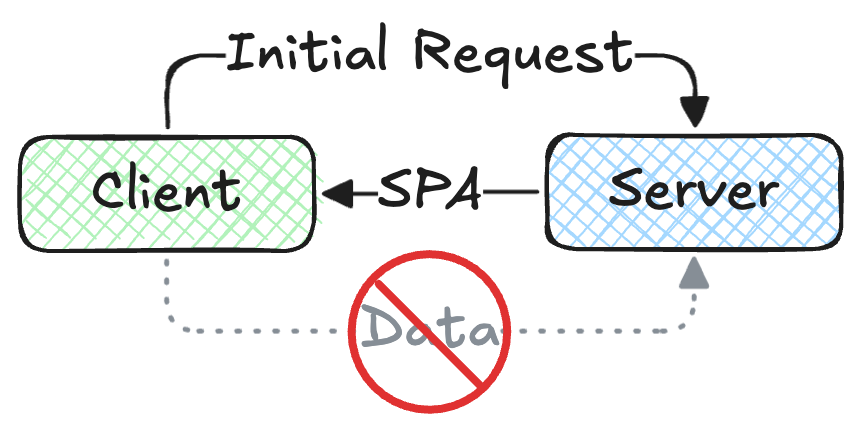
\includegraphics[width=0.5\textwidth]{../assets/privacy_illustrated.png}
    \caption{Privacy Illustrated}\label{fig:privacy_illustrated}
\end{figure}

\subsection{Usability}\label{subsec:usability}
In order to best understand the targeted user base, the project team identified personas~\fullref{subsubsec:personas}.
Using this specification, the project team created prototypes for the user interface as well as the PDF report generated by the application~\fullref{subsubsec:ux_prototyping}.

\subsubsection{Personas}\label{subsubsec:personas}
Noise is a problem almost every demographic can be affected by.
Nonetheless, the project team has attempted to capture the most common attributes of people likely to use the application. \\
\begin{table}[H]
    \centering
    \begin{tabularx}{\textwidth}{l X}
        \toprule
        \textbf{Name}           & Daniel                                                                                                                      \\
        \midrule
        \textbf{Age}            & 42                                                                                                                          \\
        \midrule
        \textbf{Sex}            & Male                                                                                                                        \\
        \midrule
        \textbf{Occupation}     & Business consultant                                                                                                         \\
        \midrule
        \textbf{Marital Status} & Married \& has two young children                                                                                           \\
        \midrule
        \textbf{Lifestyle}      & Daniel usually has to get up early in the morning because his
        customers are spread across the entire German-speaking part of Switzerland, and they expect him to meet them in their offices.                        \\
        \midrule
        \textbf{Goals}          & Daniel wants to expand his client base in hopes of possibly quitting at his workplace and founding his own consulting firm. \\
        \midrule
        \textbf{Frustrations}   & Daniel needs a lot of sleep which has been difficult ever since his first child was born.
        Much worse however, is that his new upstairs neighbors are up late every night, playing loud music,
        stomping across the floor, or arguing loudly. Daniel has already asked them to be more considerate but to no avail.                                   \\
        \midrule
        \textbf{Expectations}   & Daniel expects to find a way to prove to the police that his neighbors are consistently
        breaking the law and interfering with his and his families' lives. He expects this solution to be free, easy to use, and reliable.                    \\
        \bottomrule
    \end{tabularx}
    \caption{Persona 1 (Daniel)}\label{table:persona1}
\end{table}

\begin{table}[H]
    \centering
    \begin{tabularx}{\textwidth}{l X}
        \toprule
        \textbf{Name}           & Julia                                                                                                                \\
        \midrule
        \textbf{Age}            & 25                                                                                                                   \\
        \midrule
        \textbf{Sex}            & Female                                                                                                               \\
        \midrule
        \textbf{Occupation}     & Student                                                                                                              \\
        \midrule
        \textbf{Marital Status} & Single                                                                                                               \\
        \midrule
        \textbf{Lifestyle}      & During the day Julia is mostly attending lectures at university, running errands, or going after one of her hobbies.
        In the evenings she studies, often long into the night.                                                                                        \\
        \midrule
        \textbf{Goals}          & Julia wants to land a scholarship at a prestigious university, meaning she has to be top of her class.               \\
        \midrule
        \textbf{Frustrations}   & Julia's apartment has windows facing a busy street, and she regularly faces difficulties focussing on her studies
        due to the noise. She is convinced her landlord has neglected to install the noise isolation required by law.                                  \\
        \midrule
        \textbf{Expectations}   & Julia is looking for a way to make her landlord install better noise isolation to the apartment complex so she and
        her neighbours can spend their evenings without being bothered by the noise of passing cars and trucks.                                        \\
        \bottomrule
    \end{tabularx}
    \caption{Persona 2 (Julia)}\label{table:persona2}
\end{table}

\subsubsection{Process Model}\label{subsubsec:process_model}
The project team has created the following process model~\autoref{fig:process_model}, which is a high level illustration of how the application should work.

\begin{figure}[H]
    \centering
    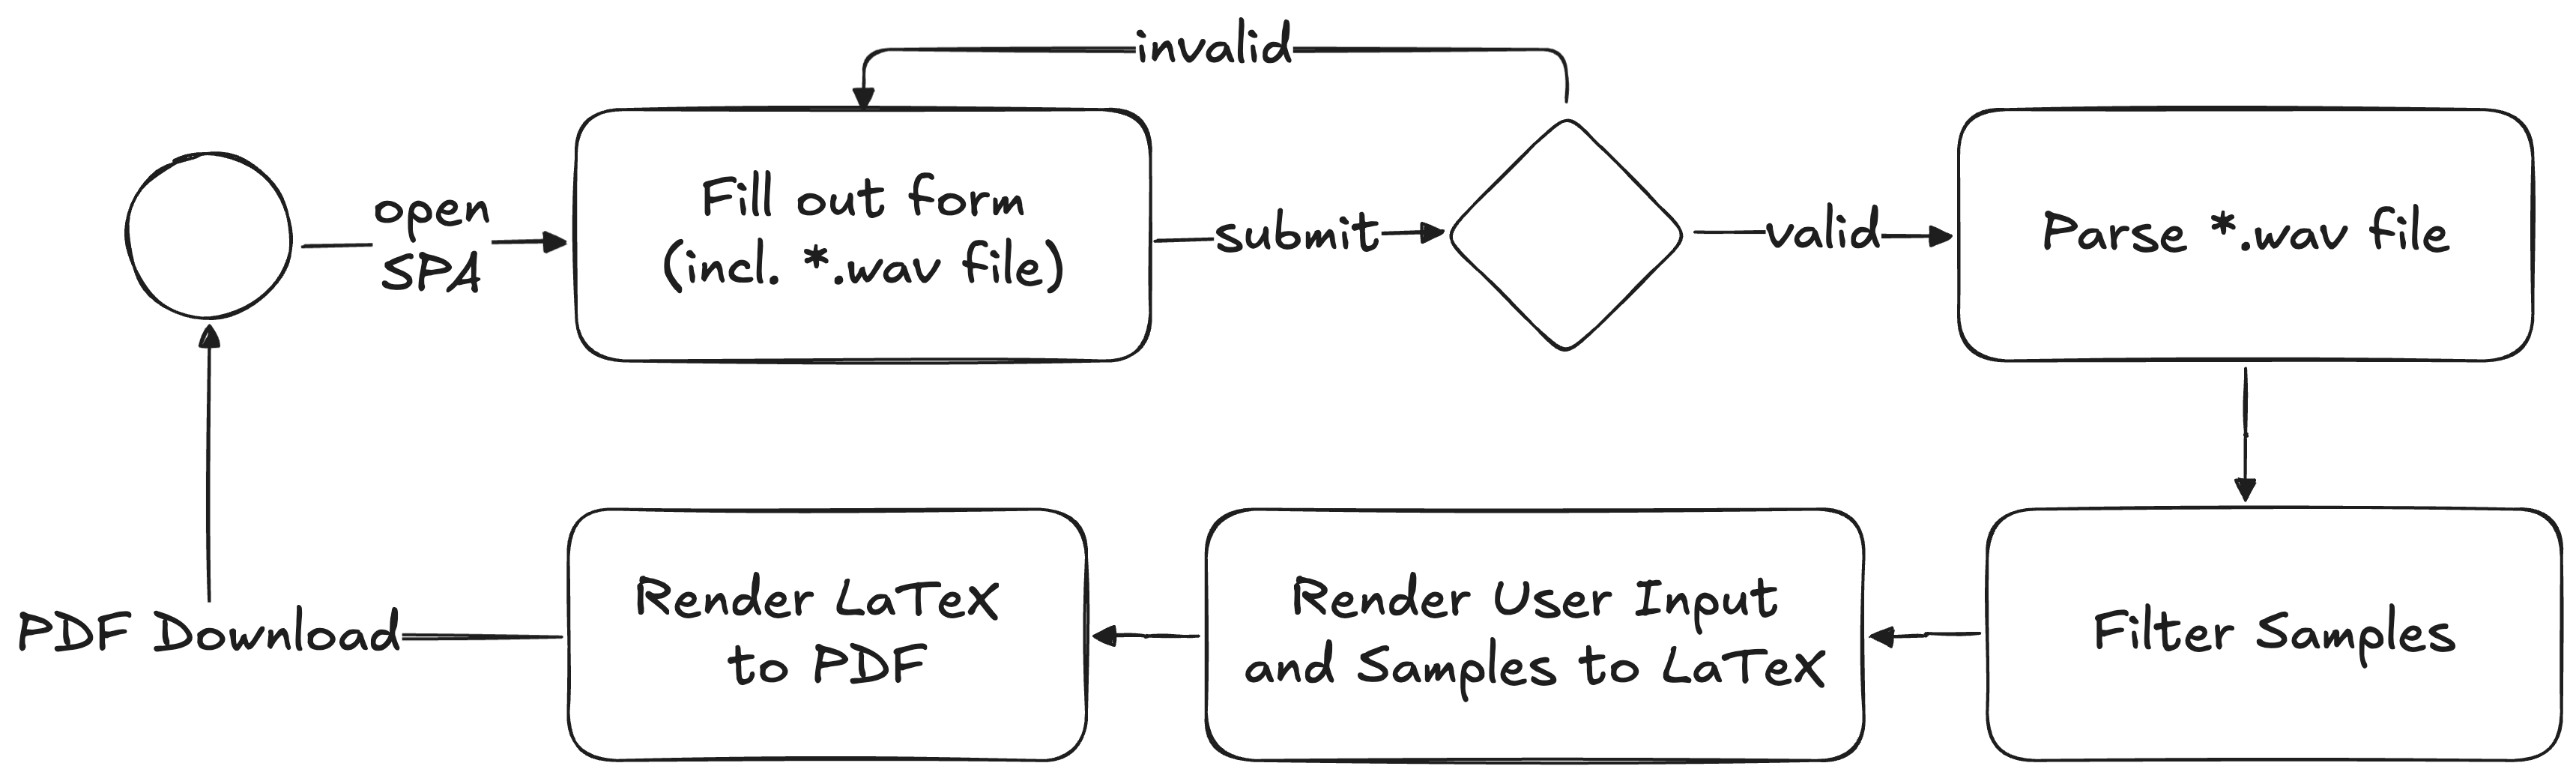
\includegraphics[width=1\textwidth]{../assets/process_model.png}
    \caption{Process Model}\label{fig:process_model}
\end{figure}

\subsubsection{UX-Prototyping}\label{subsubsec:ux_prototyping}
Based on the functional requirements~\fullref{subsubsec:functional_requirements} and the process model~\autoref{fig:process_model}, the project team identified two main UX components of the application and created their respective UX-Prototypes:
\begin{itemize}
    \item UX Prototype – Website~\autoref{fig:ux_prototype_website},~\autoref{fig:ux_prototype_website_tooltips}
    \item UX Prototype – PDF Report~\autoref{fig:ux_prototype_pdf_report}
\end{itemize}

\begin{figure}[H]
    \centering
    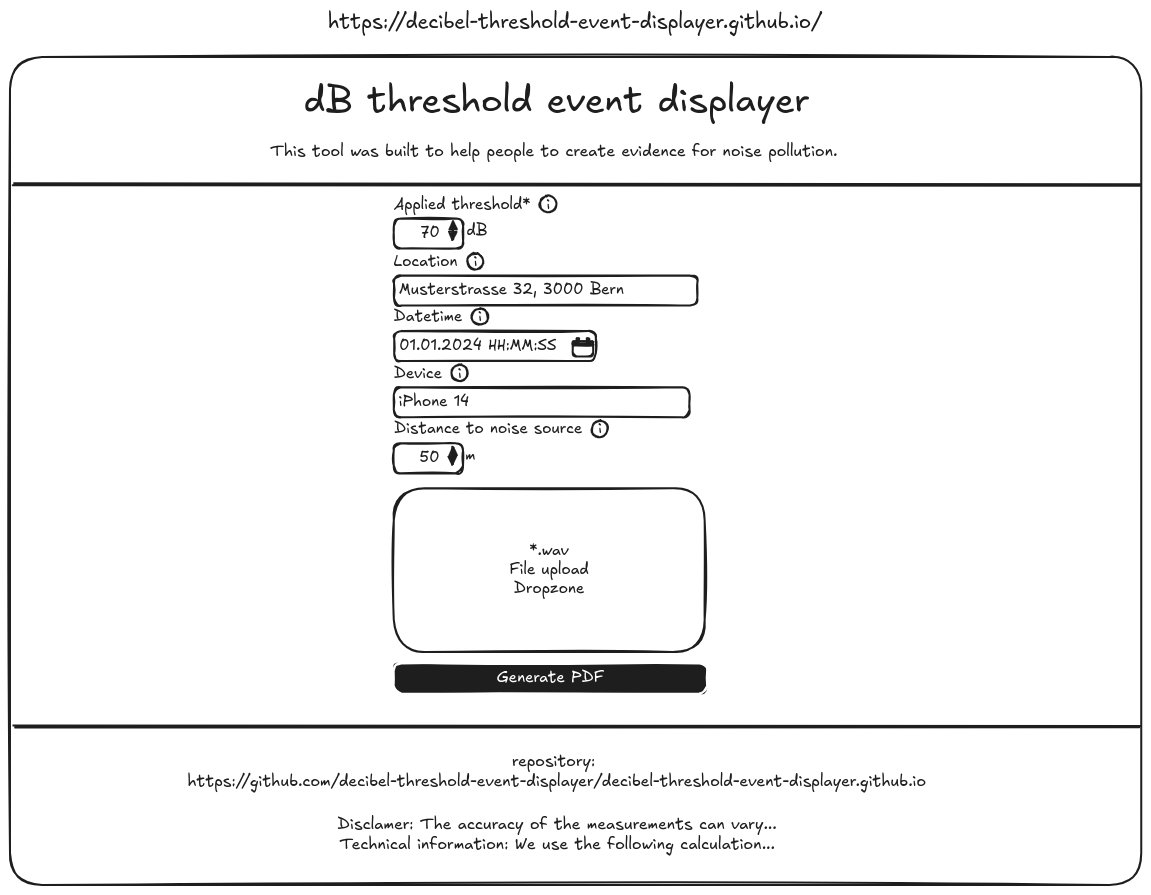
\includegraphics[width=1\textwidth]{../assets/ux_prototype_website.png}
    \caption{UX Prototype – Website}\label{fig:ux_prototype_website}
\end{figure}

\begin{figure}[H]
    \centering
    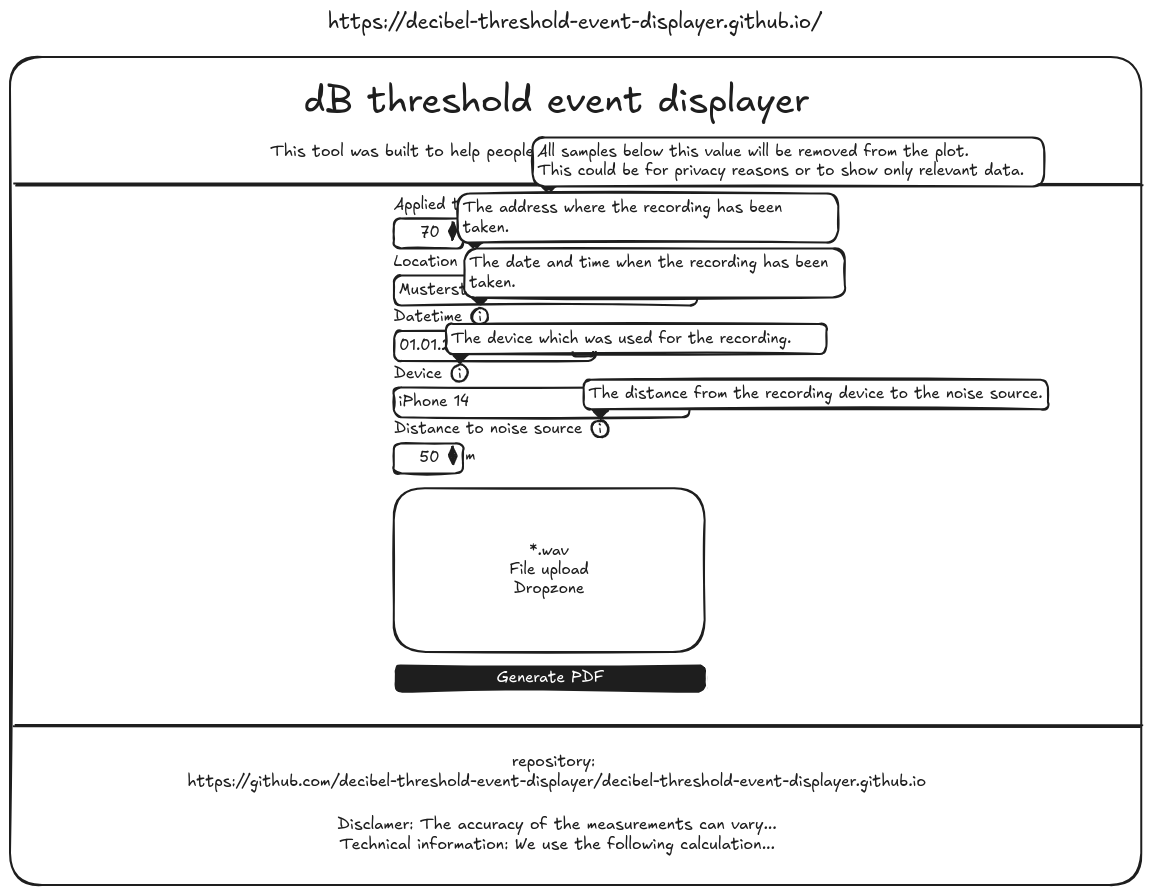
\includegraphics[width=1\textwidth]{../assets/ux_prototype_website_tooltips.png}
    \caption{UX Prototype – Website with open tooltips}\label{fig:ux_prototype_website_tooltips}
\end{figure}

\begin{figure}[H]
    \centering
    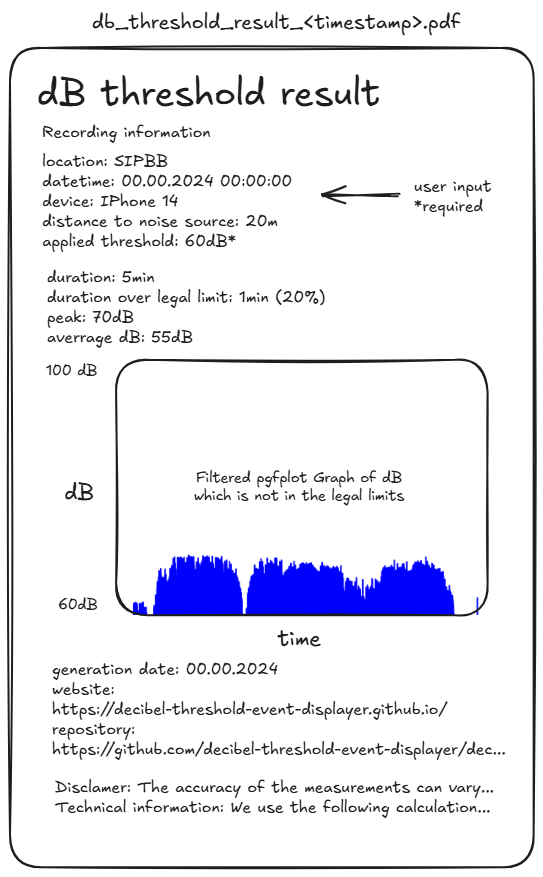
\includegraphics[width=0.9\textwidth]{../assets/ux_prototype.png}
    \caption{UX Prototype – PDF Report}\label{fig:ux_prototype_pdf_report}
\end{figure}

